\documentclass[border=5pt]{standalone}
\usepackage{tikz}
\usepackage{amsmath}
\begin{document}
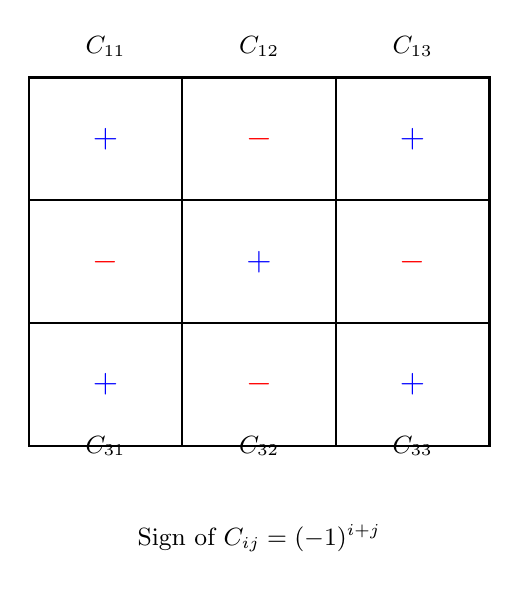
\begin{tikzpicture}[scale=1.3, >=stealth]
  % Cofactor sign pattern (checkerboard)

  % Grid
  \foreach \i in {0,1,2} {
    \foreach \j in {0,1,2} {
      \draw[thick] (\j*1.5, -\i*1.2) rectangle (\j*1.5+1.5, -\i*1.2+1.2);
    }
  }

  % Signs: + - + / - + - / + - +
  \node[font=\large, blue] at (0.75, 0.6) {$+$};
  \node[font=\large, red] at (2.25, 0.6) {$-$};
  \node[font=\large, blue] at (3.75, 0.6) {$+$};

  \node[font=\large, red] at (0.75, -0.6) {$-$};
  \node[font=\large, blue] at (2.25, -0.6) {$+$};
  \node[font=\large, red] at (3.75, -0.6) {$-$};

  \node[font=\large, blue] at (0.75, -1.8) {$+$};
  \node[font=\large, red] at (2.25, -1.8) {$-$};
  \node[font=\large, blue] at (3.75, -1.8) {$+$};

  % Labels
  \node[font=\small] at (0.75, 1.5) {$C_{11}$};
  \node[font=\small] at (2.25, 1.5) {$C_{12}$};
  \node[font=\small] at (3.75, 1.5) {$C_{13}$};

  \node[font=\small] at (0.75, -2.4) {$C_{31}$};
  \node[font=\small] at (2.25, -2.4) {$C_{32}$};
  \node[font=\small] at (3.75, -2.4) {$C_{33}$};

  % Formula
  \node[font=\small] at (2.25, -3.3) {Sign of $C_{ij} = (-1)^{i+j}$};
\end{tikzpicture}
\end{document}
